\documentclass{article}

\usepackage{amsthm}
\usepackage{amsmath}
\usepackage{amssymb}
\usepackage{amsfonts}

\usepackage{natbib}
\usepackage{hyperref}
\bibliographystyle{chicago}

\newcommand{\eref}[1]{(\ref{eq:#1})}
\newcommand{\fref}[1]{Fig.~\ref{fig:#1}}

\usepackage{color}
\newcommand{\comment}[3]{\textcolor{#1}{\textbf{[#2: }\textsl{#3}\textbf{]}}}
\newcommand{\swp}[1]{\comment{magenta}{SWP}{#1}}

\newcommand{\tsub}[2]{#1_{{\textrm{\tiny #2}}}}

\usepackage{graphicx}

\begin{document}
\begin{titlepage}
   \begin{center}
       \vspace*{1cm}
 
       \textbf{Estimating time-varying transmission rates of the SIR model}
 
       \vspace{1.5cm}
 
       \textbf{Sang Woo Park}
 
       \vfill
 
       supervised by \\ \vspace{0.2cm}
       Dr. Ben Bolker
       
 	   \vspace{1.5cm}
 
       A thesis presented for Math 4P06\\
 
       \vspace{0.8cm}
 
       Department of Mathematics \& Statistics\\
       McMaster University\\
       \today
 
   \end{center}
\end{titlepage}
\pagebreak

\begin{center}
\textbf{Abstract}
\end{center}

\pagebreak

\begin{center}
\textbf{Acknowledgements}
\end{center}

I would like to thank Dr. Ben Bolker and Dr. Jonathan Dushoff for their guidance throughout my undergradute studies.

I would also like to thank Mac-Theobio group.

Finally, I would like to thank my family for supporting me.

\pagebreak

\tableofcontents

\pagebreak

\section{Introduction}

Over the last few decades, a plethora of computational tools have been developed to study irregular patterns observed in epidemic time series, such as those of measles.
Central to these studies are mechanistic models, which are sets of equations that represent our understanding of the underlying biological system \citep{breto2009time}.
Mechanistic modeling of disease dynamics allows us to study the qualitative dynamics of a system and infer underlying process that drove the observed patterns in the data.
For example, we now know that the complex dynamics of measles outbreaks are driven by seasonal transmission patterns \citep{earn2000simple, dalziel2016persistent}.

%% read https://www.ncbi.nlm.nih.gov/pmc/articles/PMC2607466/
Major challenges in epidemiological modeling come from developing the actual model and parameterizing it.
One must make an appropriate set of assumptions to balance generality, realism, and precision \citep{levins1966strategy}.
These assumptions may depend on a system as well as an inferential tool.
Fortunately, a simple epidemic model, such as the Susceptible-Infected-Recovered (SIR) model can describe the measles dynamics sufficiently well \citep{earn2000simple, krylova2013effects, hempel2015century, dalziel2016persistent}.
Focusing on a simple, well-understood model allows us to make a fair comparison between different statistical methods in their ability to estimate underlying parameters;
if any changes have to be made to the model to apply a statistical tool, they will be relatively easy to understand and control.
Here, we focus on estimating the time-varying transmission rate of the SIR model.

One way to estimate the transmission rate is by matching the deterministic trajectory of the system with the observed data by minimizing their ``distance'', often measured by the sum of squares difference or negative log-likelihood \citep{riley2003transmission, chowell2004basic}.
This method of fitting a deterministic model (often referred to as trajectory matching) effectively assumes that \emph{all} variation in data can be explained by observation error alone \citep{bolker2008ecological}.
Likewise, it is possible to match gradients of the system \eref{sir} with the observed gradient, which can be estimated by fitting a smooth curve to a time series, such as piecewise polynomials, and taking its derivative \citep{ellner2002fitting}.
These methods are computationally efficient and easy to implement.

Monte Carlo methods are computationally demanding but allow us to model \emph{all} sources of variation (e.g., observation, demographic, and environmental stochasticity) explicitly.
In particular, Sequential Monte Carlo methods (also known as particle filtering) has been successfully applied in mechanistic analyses of epidemic time series \citep{he2009plug, he2011mechanistic, didelot2017model}; its ability to approximate the likelihood through a series of simulations provides a powerful technique for testing hypotheses and inferring underlying parameters \citep{ionides2006inference, breto2009time, king2015statistical}.
Approximate likelihood obtained by particle filtering can be maximized by iterated filtering \citep{ionides2011iterated, ionides2015inference} or can be incorporated into a Bayesian scheme as a particle Monte Carlo Markov Chain (MCMC) \citep{andrieu2010particle}.

Unlike any of the previously discussed methods, which can be used to estimate parameters of a wide range of systems, the time series SIR (TSIR) method seeks to estimate time-varying transmission rates of fully immunizing childhood infections, specifically \citep{finkenstadt2000time}.
The TSIR method first estimates the dynamics of the susceptible population based on the assumption that all individuals eventually become infected;
conditional on the estimated susceptible dynamics, transmission rates can be estimated using a regression. 
Even though the TSIR method is designed to tackle a specific kind of problems, it has been consistently used since its introduction.
\swp{Add more.}
So what makes it work so well?

\swp{Come back}
The main purpose of this project is to compare the TSIR method against other methods.
We begin by discussing types of epidemic time series (incidence, prevalence, mortality) and necessary assumptions behind each method, including TSIR.
Then, we compare their ability to estimate transmission rates by testing them against simulations.
Finally, we provide practical guidance for estimating parameters of the SIR model.

\section{Methods}

\subsection{SIR model}

The Susceptible-Infected-Recovered (SIR) model is one of the most basic epidemic models \citep{kermack1927contribution}.
It describes how disease spreads in a homogeneously mixing population.
Here, we present the model as a set of ordinary differential equations:
\begin{equation}\label{eq:sir}
\begin{aligned}
\frac{dS}{dt} &= b(t) - \left(\beta(t) \frac{I}{N} + \mu \right) S\\
\frac{dI}{dt} &= \beta(t) S \frac{I}{N} - (\gamma + \mu) I\\
\frac{dR}{dt} &= \gamma I - \mu R
\end{aligned}
\end{equation}
where $S$ is the number of susceptible individuals, $I$ is the number of infected individuals, and $R$ is the number of recovered (or removed) individuals.
We assume that individuals enter the susceptible pool at a rate $b(t)$.
Susceptible individuals become infected at a rate of $\beta(t)$ by contacting infected individuals.
Infected individuals recover at a rate of $\gamma$;
in other words, the infectious period is exponentially distributed with mean $1/\gamma$ time units.
Finally, all individuals experience natural mortality at a rate of $\mu$.

Here, we mainly consider two sets of stochastic simulations: (1) a single outbreak with constant transmission rate (and no movement in and out of the susceptible population) and (2) recurrent outbreaks driven by sinusoidal transmission rates.
To simulate a single outbreak, we use the following parameterization: $\beta(t) = 2, \gamma=1, \mu=b(t) = 0, N=100000$.
Initial conditions are specified as follows: $I(0) = 10$ and $S(0) = N - I(0)$.
To simulate recurrent outbreaks, we use the following parameterization: $\beta(t) = b_0 (1 + b_1 \cos (t/26 \times 2\pi)), b_0 = 500/26, b_1 = 0.15, \gamma = 1, \mu=1/(50 \times 26), N=5000000, b(t) = \mu N$. 
Initial conditions are specified as follows: $I(0) = 1 \times 10^{-4} \times N$ and $S(0) = 0.05 \times N$.
Parameters for recurrent epidemics are chosen to approximately match the parameters used in \cite{earn1998persistence}, which yields a persistent biennial cycle.
Note that $\gamma$ is scaled to 1 to represent one generation; for measles, $1/\gamma$ will have a unit of biweeks (14 days).
Stochastic simulation of the SIR model is performed using the Gillespie algorithm \citep{gillespie1976general}.

\subsection{Epidemic time series}

Epidemic time series can be broadly classified into three categories: incidence, mortality, and prevalence.
Incidence is defined as the number of newly infected individuals generated over a reporting period.
Then, true incidence of the SIR model \eref{sir} between time $t$ and $t-\tsub{t}{rep}$, where $\tsub{t}{rep}$ is the length of reporting time step, can be obtained by integrating total infection rate over the reporting period:
\begin{equation}
i_t = \int_{t-\tsub{t}{rep}}^{t} \beta(s) S \frac{I}{N} ds.
\end{equation}
Similarly, true mortality, which is defined as the number of individuals that died (or recovered for measles) during a reporting period, can be obtained by integrating total death rate over the reporting period:
\begin{equation}
m_t = \int_{t-\tsub{t}{rep}}^{t} \gamma I ds.
\end{equation}
Finally, prevalence is defined as the number of infected individuals that are present in the population; 
this corresponds to the state variable $I$. 
Incidence, mortality, and prevalence for a stochastic simulation are defined in the same manner.

Reported incidence, mortality, and prevalence cases are drawn from a beta-binomial distribution with reporting rate $\rho$, dispersion parameter $\tsub{\theta}{rep}$, and their corresponding true values \citep{morris1997disentangling}.
Unless noted otherwise, we use $\tsub{\theta}{rep} = 10$ throughout simulations.
Here, we assume that cases are reported instantaneously; 
a more realistic model can incorporate a delay between infection time and reporting time (e.g., infected individuals are likely to report after symptom onset but before recovery).
We do not explore these ideas explicitly.

Instead, we focus on how different assumptions about an epidemic time series (whether it represents incidence, mortality, or prevalence) affect our inference.
While this question was initially motivated by the TSIR framework, in which incidence is assumed to be equal to prevalence when reporting time is equal to mean generation time, 
misclassification of epidemic time series is not rare.
For example, \cite{he2009plug} assume that incidence is measured upon recovery whereas \cite{hooker2010parameterizing, althaus2014estimating} assume that incidence is measured upon transition from latent to infectious period.
Understanding these differences is crucial in order to correctly estimate underlying parameters as well as their associated uncertainties.
For all other purposes, we use the incidence time series throughout this study.

\subsection{Fitting methods}

\subsubsection*{Time-series SIR model}

The time-series SIR (TSIR) method was developed by \cite{finkenstadt2000time} to estimate seasonally varying transmission rates of measles.
The TSIR method begins by discretizing the infection process of the SIR model, assuming that disease generation time is equal to reporting interval:
\begin{equation}\label{eq:tsir_dynamics}
\begin{aligned}
S_{t+1} &= B_t + S_t - i_{t+1}\\
i_{t+1} &= \beta_t S_t \frac{i_t^\alpha}{N_t}
\end{aligned}
\end{equation}
where $\alpha$ is often referred to as a conversion factor for discretization of a system or inhomogeneity \citep{liu1986influence, bjornstad2002dynamics, glass2003interpreting}.
Taking log on both sides, estimation of the transmission rates $\beta_t$ becomes a regression problem:
\begin{equation}\label{eq:tsir}
\log i_{t + 1} = \log \beta_t + \log S_t + \alpha \log i_t - \log N_t + \epsilon_t.
\end{equation}

A key assumption behind the TSIR model is that all, if not most, individuals become infected eventually \citep{finkenstadt2000time}.
In other words, the total number of births should be equal to the total number of cases over a long period of time.
Rewriting true incidence $i_t$ as a product of reported cases $i_{t, {\tiny \textrm{rep}}}$ and reciprocal of reporting rate $1/\rho_t$ and iteratively solving \eref{tsir_dynamics}, we get
\begin{equation}
\sum_{t=1}^N B_t = \sum_{t=1}^N \frac{i_{t, {\tiny \textrm{rep}}}}{\rho_{t+1}} + Z_{t+1} - Z_1,
\end{equation}
where $Z_t = S_t - \bar{S}$.
Under this assumption, fitting a regression model to cumulative birth as a function of cumulative cases allows us to estimate time-varying reporting rate $\rho_t$ by taking the reciprocal of the slope and susceptible dynamics $Z_t$ from the residuals \citep{finkenstadt2000time}.
Conditioning on the known susceptible dynamics, we can apply the TSIR regression \label{eq:tsir} to epidemic time series to estimate the time-varying transmission rate.

\subsubsection*{Trajectory matching}

Trajectory matching is a way of estimating underlying parameters of an ODE model by matching the observed time series and a deterministic solution of the model.
Given observed incidence $i_{t, {\tiny \textrm{rep}}}$ (or equivalently, observed prevalence or mortality), we can define its expected dynamics using the solution of the SIR model:
\begin{equation}
\mu_t = \rho i_t = \rho \int_{t-\tsub{t}{rep}}^{t} \beta(s) S \frac{I}{N} ds,
\end{equation}
where $\rho$ is the mean reporting rate.
Directly computing this integral is practically infeasible. 
Instead, we can include an extra state variable $C$ which represents cumulative number of cases to the SIR model: $dC/dt = \beta SI/N$.
True incidence can be calculated by taking the difference of $C$ between to consecutive reporting periods.
Then, we get
\begin{equation}
\mu_t = \rho (C(t) - C(t-\tsub{t}{rep})).
\end{equation}
Finally, the observation likelihood can be defined as a deviation from this mean trajectory:
\begin{equation}
i_{t, {\tiny \textrm{rep}}} \sim \mathrm{NegBin}(\mu_t, \tsub{\phi}{obs}),
\end{equation}
where $\tsub{\phi}{obs}$ is the dispersion parameter of a negative binomial distribution.

\swp{Maybe come back.}

\subsubsection*{Gradient matching}

Like trajectory matching, gradient matching seeks to find a set of parameters such that the gradient of an ODE model matches the observed gradient \citep{ellner2002fitting}.
Gradient matching provides a flexible way of modeling a system as it does not require the parametric form of the rate equations to be pre-specified (e.g., we do not need to assume that per-capita rate of transmission is a linear function of $I$).
Instead, parameters can be estimated by fitting a non-parametric regression model to the observed gradient as a function of relevant state variables.
Therefore, all state variables must be observed in order to apply gradient matching.

In practice, it is difficult to observe all state variables of an epidemic model, even for simple models such as the SIR model.
When either incidence or mortality are reported, \emph{no} relevant state variables are observed.
Nonetheless, it is still possible to estimate the transmission rates of the SIR model using gradient matching by making similar assumptions as the TSIR model.
Here, we briefly outline the estimation process;
note that the purpose of this section is to introduce the method, rather than to provide a rigorous justification of the statistical model.

First, we begin by assuming that the mean generation time is equal to the length of reporting time step and that incidence is proportional to prevalence, i.e., $i_t = a I_t$ for some $a > 0$. 
This assumption is slightly weaker than the conditions for the TSIR method.
We then fit a smooth curve $f(t)$ to log reported incidence $\log i_{t, {\tiny \textrm{rep}}}$:
\begin{equation}
\log i_{t, {\tiny \textrm{rep}}} \sim \mathrm{Normal}\left(f(t), \tsub{\sigma}{smooth}^2 \right),
\end{equation}
where natural cubic splines are used to model the function $f$.
For the purpose of estimating time-varying transmission rates, placing basis knots every 6 generations appear to be sufficient \swp{Appendix}.

The smooth curve $f(t)$ represents the dynamics of the log of prevalence ($\log I_t$) up to a constant.
When we take the derivative of the curve $f(t_i)$, we get an estimate of the derivative of the log of prevalence:
\begin{equation}
E\left[\frac{df(t)}{dt}\right] = \beta(t) S - (\gamma + \mu),
\end{equation}
where the unobserved dynamics of the susceptible $S$ can be inferred from the susceptible reconstruction of the TSIR method.
There are several ways we can estimate the transmission rate from this equation.
First, we can model transmission rate as a function of susceptibles $S$ by fitting a non-parametric regression by treating known values of $\gamma$ and $\mu$ as offset terms:
\begin{equation}
\frac{df(t)}{dt} \sim \mathrm{Normal}(g(S_t) - (\gamma + \mu), \sigma^2),
\end{equation}
where $g$ is a non-parametric function that represents the transmission rate.
When transmission varies over time, we can either (1) model transmission rate as an interaction term between a factor variable that represents time of the year and a smoothing term (i.e., fit a separate nonparametric curve $g$ for each factor level) or try to separate transmission rate from the susceptible dynamics using a log link function:
\begin{equation}
\frac{d f(t)}{dt} + (\gamma + \mu) \sim \mathrm{Normal}\left(\exp \left(\log \beta_t + \log S_t\right), \sigma^2\right),
\end{equation}
where log number of susceptible individuals $\log S_t$ is treated as an offset term and the log transmission rate can be estimated is estimated as a function of time of year using a nonparametric regression.
Here, we mainly focus on the last method.

\subsubsection*{Sequential Monte Carlo}

Calculating the exact likelihood of a nonlinear stochastic system is practically impossible.
Instead, Sequential Monte Carlo (also known as particle filtering) allows the likelihood to be approximated via simulations \citep{doucet2001introduction, arulampalam2002tutorial}.
Let $X_t = \{\mathbf{x}_{t, i} \,|\, i= 1, 2, \dots, n\}$ be the set of states (particles) at time $t$ and $h$ be the process model.
For the SIR model, each particle $\mathbf{x}_{t, i} \in X$ will consist of the number of susceptible individuals $S_t$ and the number of infected individuals $I_t$.
Then, we can predict the state of each particle at next time reporting step $t+1$ using the process model: $h(\mathbf{x}_{t, i})$.
Note that it may take several \emph{simulation} time steps to get to the next reporting time step.
For each prediction $h(\mathbf{x}_{t, i})$, we can calcuate the likelihood $w_{t,i}$ of the observation at time $t+1$ and define marginal likelihood by taking the average: $\bar{w}_t$.
Then, drawing $n$ weighted samples from the set $\{h(\mathbf{x}_{t, i}) \,|\, i = 1=2, \dots, n\}$, where the weight of each $h(\mathbf{x}_{t, i})$ is proportional to $w_i$, yields the next set of particles $X_{t+1}$.
This algorithm can be repeated until the final reporting time step.
Finally, the complete likelihood of the data is given by the product of the marginal likelihood at each time step: $\prod \bar{w}_{t}$.

While Sequential Monte Carlo provides a straightforward way of approximating the likelihood for any process model that can be defined, it is still difficult fit a continuous-time stochastic model. 
For example, it can take as long as 10 hours to simulate a measles times series for 20 years with a gillspie algorithm.
Computing a likelihood with large number of particles will take more than a few days; 
maximizing the likelihood will be practically impossible.

Instead of fitting a continuous-time model, we can assume that an epidemic process is a partially observed discrete-time Markov process and discretize the system by using a hazard approximation to the transition probabilities between states:
\begin{equation}
\begin{aligned}
B(t) &\sim \mathrm{Poisson}(b(t) \Delta t)\\
F_{S}(t) &\sim \mathrm{Binomial}(S_t, 1 - \exp(- (r_1 + r_2) \Delta t))\\
F_{I}(t) &\sim \mathrm{Binomial}(I_t, 1 - \exp(- (r_3 + r_4) \Delta t))\\
F_{S,I}(t) &\sim \mathrm{Binomial}\left(F_{S}(t), \frac{r_1}{r_1 + r_2}\right)\\
S(t+\Delta t) &= B(t) + S(t) - F_{S}(t) \\
I(t+\Delta t) &= F{S,I}(t) + I(t) - F_{I}(t)\\
C(t+\Delta t) &= C(t) + F{S,I}(t)\\
\end{aligned}
\end{equation}
where $r_1 = \beta I/N$, $r_3 = \gamma$, and $r_2 = r_4 = \mu$.
$\Delta t$ represents simulation time step; as $\Delta t \to 0$, this model converges to a Gillespie simulation.
Random variables $F_S(t)$ and $F_I(t)$ represent the total number of individuals that move out from susceptible $S$ and infected $I$ states. 
Likewise, $F_{S, I}(t)$ represent the total number of individual move from susceptible state $S$ to infected state $t$.
Finally, the state variable $C(t)$ keeps track of cumulative incidence.
Again, we define observation likelihood using a negative-binomial distribution:
\begin{equation}
i_{t, {\tiny \textrm{rep}}} \sim \mathrm{NegBin}(\rho (C(t) - C(t - \tsub{t}{rep})) , \tsub{\phi}{obs}).
\end{equation}
This model is implemented in the R package \texttt{POMP} \citep{king2015statistical}.

\subsubsection*{Renewal equation}

Many standard compartmental models, such as the SIR model, assume that the shape of generation-interval distribution is known exactly.
The continuous-time SIR model assumes that generation intervals are exponentially distributed.
The discrete-time SIR model represented as a partially observed Markov process assumes that generation intervals are geometrically distributed.
Finally, the TSIR model assumes that generation intervals are fixed.
We expect a realistic generation-interval distribution of measles to be narrower than exponential but not fixed.
While it is possible to use differently shaped generation-interval distributions by incrementing the number of compartments used for each state, the number of compartments has to be specified prior to model fitting.

Instead, renewal equation allows us to model incidence as a function of a previous incidence and generation-interval distributions explicitly:
\begin{equation}
i(t) = \mathcal R_0 S(t) \int_0^t g(t-s) i(s) ds,
\end{equation}
where $i(t)$ represents incidence, $S(t)$ represents number of susceptible individuals, $g(t)$ represents generation-interval distribution and $\mathcal R_0$ represents the basic reproductive number.
Because the renewal equation generalizes the compartmental models with Erlang distributed latent and infectious periods (i.e., models with multiple latent and infectious compartments), including the standard SIR model \citep{champredon2018equivalence}, we expect this model to perform better in analyzing time series of outbreaks.

Previous studies used a discrete time version of the renewal equation model to analyze Ebola epidemics but assumed that the simulation time step was equal to the reporting time step \citep{li2018fitting, champredon2018two}.
Here, we extend their models by relaxing this assumption and allowing for natural birth and death in the susceptible population:
\begin{equation}
\begin{aligned}
B(t) &\sim \mathrm{Poisson}(b(t) \Delta t)\\
\phi(t) &= \mathcal R(t) \sum_{k=1}^\ell i(t - (k-1) \Delta t) g(k \Delta t)\\
F_{S}(t) &\sim \mathrm{Binomial}\left(S(t), 1 - e^{-(\phi(t) + \mu \Delta t)} \right)\\
i(t + \Delta t) &\sim \mathrm{Binomial}\left(F_{S}(t), \frac{\phi(t)}{\phi(t) + \mu \Delta t} \right)\\
S(t + \Delta t) &= B(t) + S(t) - F_{S}(t)
\end{aligned}
\end{equation}
This model can be fitted using a Bayesian machine such as JAGS \citep{plummer2003jags}, NIMBLE \citep{de2017programming}, and Stan \citep{carpenter2017stan} (see \cite{li2018fitting} for comparison across these platforms).

In order to make a fair comparison (without relying on a Bayesian prior), we take a further step to translate this model into a Markov process such that it can be used with particle filtering.
We define a set of new state variables $j_1, j_2, \dots, j_\ell$ such that $j_k(t)$ corresponds to $i(t- (\ell-k) \Delta t)$.
Then, we can rewrite the model as follows:
\begin{equation}
\begin{aligned}
B(t) &\sim \mathrm{Poisson}(b(t) \Delta t)\\
\phi(t) &= \mathcal R(t) \sum_{k=1}^\ell j_{\ell-k+1}(t) g(k \Delta t)\\
F_{S}(t) &\sim \mathrm{Binomial}\left(S(t), 1 - e^{-(\phi(t) + \mu \Delta t)} \right)\\
j_k(t+\Delta t) &= j_{k+1}(t) &k=1, 2, \dots, \ell-1\\
j_\ell(t + \Delta t) &\sim \mathrm{Binomial}\left(F_{S}(t), \frac{\phi(t)}{\phi(t) + \mu \Delta t} \right)\\
S(t + \Delta t) &= B(t) + S(t) - F_{S}(t)
\end{aligned}
\end{equation}
\swp{Write down likelihood}

We model the generation-interval distribution using a negative binomial distribution:
\begin{equation}
g(t) \propto t^{\tsub{G}{shape}} \exp(-t/\tsub{G}{scale}),
\end{equation}
where $g(t)$ is normalized to sum to one.
For estimation purposes, we use an alternate parameterization $(\tsub{G}{mean}, \tsub{G}{var})$ such that $\tsub{G}{scale} = \tsub{G}{var}/\tsub{G}{mean}$ and $\tsub{G}{shape} = \tsub{G}{mean}/\tsub{G}{scale}$.
For sufficiently small $\Delta t$, $\tsub{G}{mean}$ and $\tsub{G}{var}$ corresponds to mean and variance of the generation-interval distribution.
Here, we use a simulation time step $\Delta t$ of one-twentieth of the mean generation interval and $\ell = 120$; this allows the generation-interval distribution to span over 6 generations.

\subsection{Splines}

In order to estimate time-varying transmission rates as a smooth function of time, we model transmission rate $\beta(t)$ using a spline \citep{hooker2010parameterizing}:
\begin{equation}
\beta(t) = \sum_{i=1}^k \phi_i(t) b_i,
\end{equation}
where each $\phi_i$ is a cyclic cubic B-spline basis and $b_i$ is the corresponding coefficient.
Here, we fix knot locations at every two biweeks (1/13 years);
this parameterization results in almost a two-fold reduction in the number of parameters to be estimated compared to the regular TSIR procedure, which tries to estimate a separate transmission rate at every biweek.
For regression-based methods (TSIR and gradient matching), we allow the number of knots to be estimated within the regression method by the Restricted Maximum Likelihood (REML) approach \citep{wood2012mgcv}.

\section{Results}

\subsection{Types of epidemic time series}

When reporting step is equal to mean generation time, incidence and prevalence are often assumed to be equivalent (\fref{incidence}).
In fact, we can show that incidence, prevalence, and mortality are nearly equivalent for simple SIR model \eref{sir} under Euler approximation when reporting step is equal to mean generation time (see Appendix).
Their deterministic dynamics are sufficiently similar that we expect these three reports to be nearly indistinguishable from each other when demographic stochasticity and observation error is introduced.
However, this is not true for more complicated models.
For a more realistic model with an exposed period (SEIR model), the incidence is comparable to prevalence when reporting time step is equal to mean \emph{infectious period} rather than mean \emph{generation time}.
We are not able to see this distinction in the SIR model because it assumes that the mean infectious period is equal mean generation interval.
For now, we focus on the SIR model. 
\swp{We revisit this point in Discussion.}

\begin{figure}[!ht]
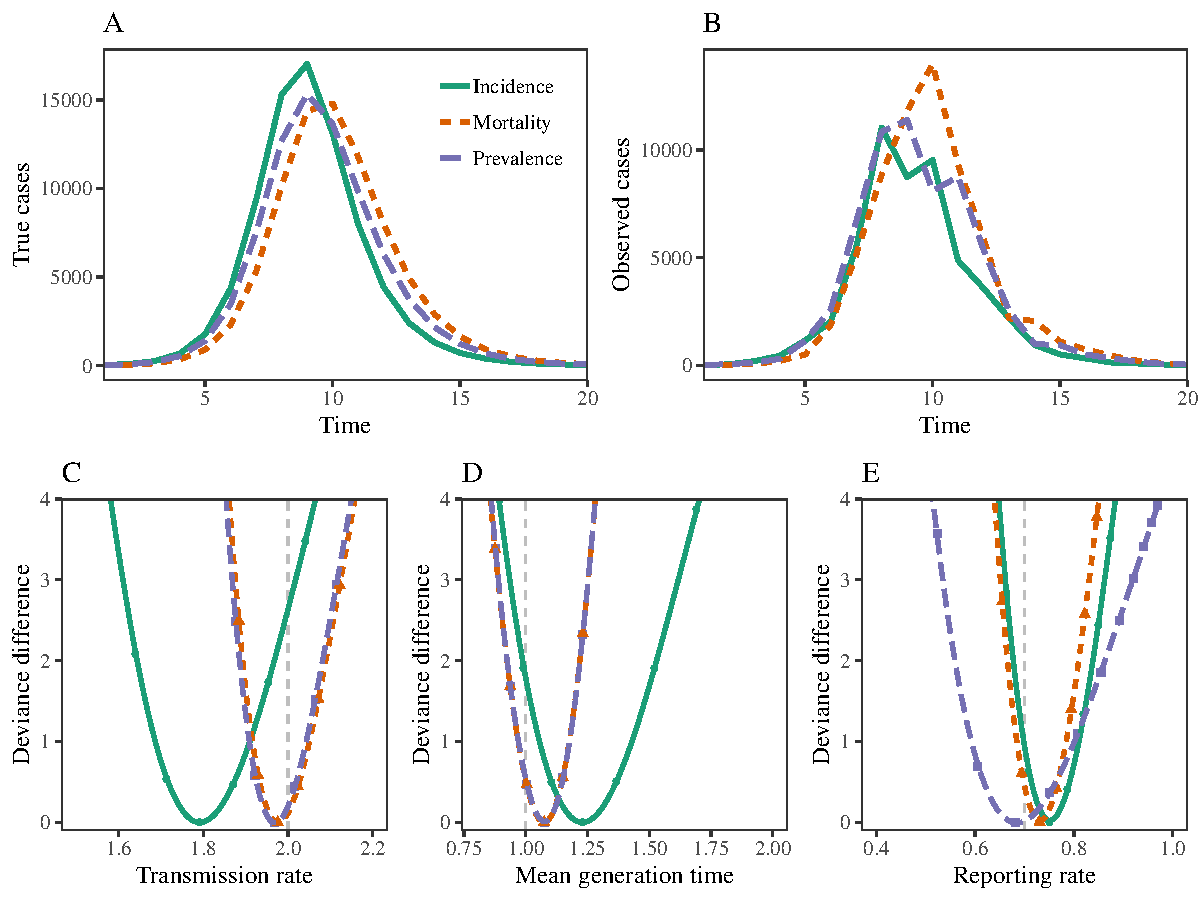
\includegraphics[width=\textwidth]{../figure/compare_profile_likelihood.pdf}
\caption{
\textbf{Comparison of incidence, prevalence, and mortality from dynamical and estimation perspective.}
A: deterministic dynamics of incidence, mortality, and prevalence of the SIR model for a single outbreak (no natural birth/death and fixed transmission rate) when mean generation time is equal to reporting step.
The parameters and initial conditions are $\beta = 2$, $\gamma = 1$, $N = 1 \times 10^5$, $I(0) = 10$, and $S(0) = N - 10$.
B: dynamics of incidence, mortality and prevalence of the SIR model with sinusoidal transmission rate ($\beta(t) = b_0 (1 + b_1 \cos (2 \pi t/26))$) when mean generation time ie equal to reporting step.
The parameters and initial conditions are $b_0 = 500/26$, $b_1 = 0.15$, $\gamma = 1$, $\mu = 1/(50 \times 26)$, $N = 5 \times 10^6$, $I(0) = 0.0001 N$, $S(0) = 0.05 N$.
C, D, E: deviance difference (profile likelihood minus the maximum likelihood) of each parameter when incidence, mortality, and prevalence are fit to same time series using trajectory matching. 
Grey dashed line represents the true value.
} 
\label{fig:incidence}
\end{figure}

Even if incidence, mortality, and prevalence exhibit similar dynamics when reporting step is equal to mean generation time, it is important to distinguish them when we are trying to estimate underlying parameters of the SIR model, especially when mean generation time $1/\gamma$ is not exactly known.
To demonstrate this idea, we first simulate an epidemic time series representing prevalence over time by solving the deterministic SIR model numerically and calculating prevalence, $I(t)$, for 20 reporting periods, where reporting period is equal to the mean generation time. Then, we draw a beta-binomial random variable at each time step with a reporting rate of 70\% and an overdispersion parameter of 10.
Using this time series, we try to estimate four parameters -- transmission rate $\beta$, recovery rate $\gamma$, reporting rate $\rho$, and an initial number of infected individuals $I(0)$ -- by treating the same time series as if it were incidence, mortality, and prevalence report (\fref{incidence}).

We find that fitting prevalence and mortality curves to the same time series yields almost identical estimates of the transmission rate $\beta$ and the recovery rate $\gamma$ (as well as related uncertainty in the estimates) whereas fitting incidence and mortality curves to the same time series yields consistent estimates of the reporting rate $\rho$.
As mortality always behaves like prevalence regardless of reporting period (reported mortality case at time $t$ is approximately equal to $\rho \gamma I(t-\tsub{t}{rep}) \tsub{t}{rep}$),
it is possible to generate a mortality curve that matches its corresponding prevalence curve by adjusting the reporting rate of $\rho$.
This explains why estimates of dynamical parameters, $\beta$ and $\gamma$, are similar whether we fit prevalence or mortality.
On the other hand, incidence report no longer matches prevalence report when reporting period is not equal to the mean generation time (i.e., when $\gamma$ is being estimated); therefore, fitting incidence curve yields a different estimate of the dynamical parameters, $\beta$ and $\gamma$, from fitting mortality or prevalence curves.
Fitting incidence and mortality curve yields similar estimates of the reporting rate $\rho$ because they both contain equivalent information about the final size of an epidemic: total \emph{true} incidence and total \emph{true} mortality is equal to the final size of an epidemic.

Even when mean generation time is exactly known, we find that estimates of transmission rate $\beta$ and reporting rate $\rho$ depends on our assumptions about the time series.
We find that fitting mortality and prevalence yields consistent estimates of both $\beta$ and $\rho$ in this case, whereas fitting incidence yields similar but still different estimates.
Treating incidence report as prevalence report (and vice versa) should be avoided.
\swp{Appendix; come back}

\subsection{Susceptible reconstruction}

One of the main assumptions behind the TSIR method is that the dynamics susceptible population $S_t$ is exactly known.
Assuming that all individuals that enter the susceptible population become infected eventually, it is possible to recover the reporting rate, $\rho_t$, as well as the dynamics of the susceptible population as a deviation from its mean, $Z_t = S_t - \bar{S}$, by fitting a regression model between cumulative births and cumulative cases: 
\begin{equation}
\sum_{t=1}^N B_t = \sum_{t=1}^N \frac{C_{t+1}}{\rho_{t+1}} + Z_{t+1} - Z_1,
\end{equation}
where $C_t$ is the number of observed cases: $C_t = \rho_t i_t$.
Then, the reporting rate $\rho_t$ can be estimated from the slope of the regression and the susceptible dynamics can be estimated from the residuals \citep{finkenstadt2000time}. 

\begin{figure}[!t]
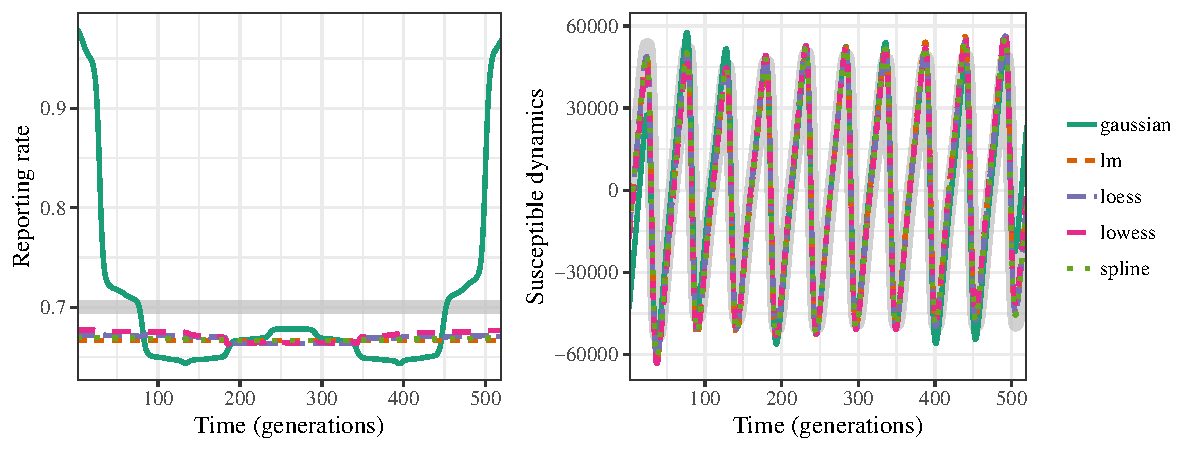
\includegraphics[width=\textwidth]{../figure/susceptible_reconstruction_tsir.pdf}
\caption{
\textbf{Sensitivity of estimates of reporting rate and susceptible dynamics to regression methods.}
Susceptible reconstruction is performed on a simulated time series (thick grey lines represent the true values).
Although estimates of the reporting rates are highly sensitive to regression methods, susceptible dynamics can be robustly estimated.
}
\label{fig:tsirrecon}
\end{figure}

While the susceptible reconstruction has been successfully used with the TSIR method, 
several minor questions remain to be answered.
First, how sensitive is our inference to regression methods?
Second, does $Z_t$ represent the deviation from the overall population mean $\bar{S}$ or from a long-term moving average (assuming that population changes over time)?
\cite{finkenstadt2000time} initially defined $Z_t$ as $S_t - \bar{S}$, but this definition was corrected to $Z_t = S_t - \sigma N_t$, where $\sigma$ is the mean proportion susceptible, by \cite{dalziel2016persistent} without justification.
Finally, how do changes in population size or reporting rate over time affect our estimate of $\rho_{t+1}$ or $Z_t$?

We first simulate an epidemic using the continuous deterministic SIR model with sinusoidal transmission rates for 10 years.
After introducing observation error base on a beta-binomial distribution, we apply 5 different regression models (Gaussian regression, linear model, locally estimated scatterplot smoothing, locally weighted scatterplot smoothing, and spline model) available from the \texttt{tsiR} package to test their ability to infer the reporting rate and susceptible dynamics (\fref{transmission}).
We find that estimates of reporting rates are highly sensitive to regression methods.
The Gaussian regression is particularly bad at estimating the reporting rates near the boundaries.
Estimates of susceptible dynamics appear to be robust regardless of the regression method.

\begin{figure}[!t]
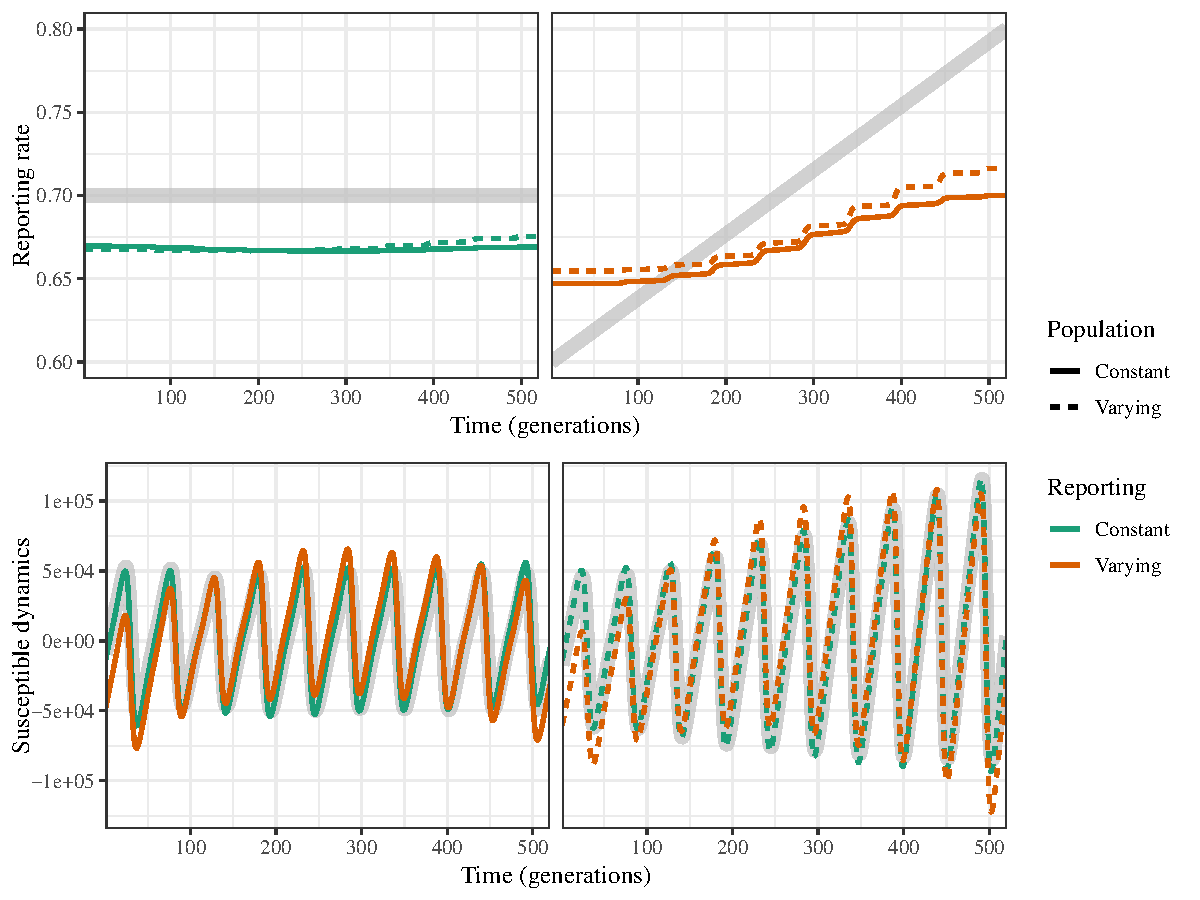
\includegraphics[width=\textwidth]{../figure/susceptible_reconstruction_compare.pdf}
\caption{
\textbf{Estimates of susceptible dynamics and reporting rate under different scenarios.}
Susceptible reconstruction is performed on a simulated time series under different scenarios (thick grey lines represent the true values).
Spline regression is used throughout these simulations.
}
\label{fig:tsircomp}
\end{figure}

We then allow for both population size and reporting to stay constant or increase over time.
Then, we compare estimates of susceptible dynamics and reporting rate under all combinations (total of 4) of these scenarios (\fref{tsircomp}).
We find that estimating time-varying reporting rate is difficult;
the increasing pattern in the reporting rate is only partially captured in the slope of the regression model.
We also find that the susceptible dynamics $Z_t$ estimated from a regression better matches $S_t - \bar{S}$ rather than $S_t - \sigma N$ (latter results are not shown).
In other words, any long-term dynamics in the susceptible population is expected to be captured in $Z_t$.

\subsection{Density dependence}

\begin{figure}
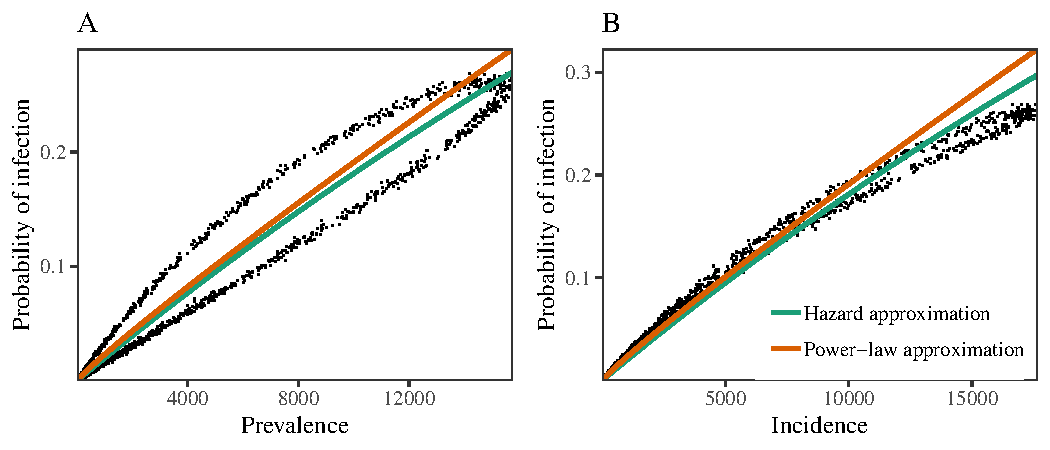
\includegraphics[width=\textwidth]{../figure/tsir_poi.pdf}
\caption{
\textbf{Density dependence of the infection process.}
A: the probability of infection over a generation as a function of prevalence.
B: the probability of infection over a generation as a function of incidence.
The hazard approximation is calculated using the true transmission rates.
The power-law approximation is calculated by fitting the TSIR model to 100 simulations.
C: ratio of next incidence $i_{t+1}$ and a power function of current incidence $i_t^{\alpha}$ as a function of the current number of susceptibles $S_t$; this relationship is expected to be linear under the TSIR framework.
Solid black line is the estimated relationship from the TSIR method when we introduce an exponent to $S_t$: $i_{t+1}/i_t^{0.92} = 4.9 S_t^{0.98}$.
Points are calculated from 100 Gillespie simulations for single outbreaks.
}
\label{fig:tsirpoi}
\end{figure}

In a continuous time SIR model, density dependence in the infection process is implicitly captured in the nonlinear infection term $\beta S I/N$.
As the number of infected individuals increases, competition among infected individuals to find a susceptible host also increases. 
This results in saturation in the probability of infection (\fref{tsirpoi}A).

The simplest way to account for density dependence in a discrete time model is to approximate the probability of infection a hazard function, $1- \exp(- \phi \Delta t)$.
This approximation can be obtained by integrating $dS/dt = - \phi S$ over $\Delta t$ assuming a constant force of infection $\phi = \beta I/N$.
While this approximation captures the \emph{average} probability of infection reasonably well, the \emph{realized} probability of infection deviates from this approximation (\fref{tsirpoi}A).
When an epidemic is growing, the force of infection increases over time, resulting in a higher realized probability of infection.
Likewise, when an epidemic is dying out, the force of infection decreases over time, resulting in a lower probability of infection.
It is still useful to model probability infection using the hazard function because it provides a probabilistic interpretation of the transition between states, which can be incorporated in stochastic models. 

On the other hand, the TSIR model assumes that the probability of infection follows a power function of the current incidence: $\hat{\beta} i_t^\alpha/N$, where $\alpha$ is a correction factor for heterogeneity or discretization of a continuous model \citep{glass2003interpreting}.
\cite{glass2003interpreting} further derived an analytical expression for the optimal value of $\alpha$ as a function of birth rate and the basic reproductive number by comparing the second order Taylor expansion of the TSIR model to that of a continuous time model.
In the absence of susceptible recruitment to the population, the optimal value of $\alpha$ based on their approximation is unity, which has been regarded as the condition for homogeneous mixing.
This is false.

Instead, we propose that $\alpha$ should be interpreted as the strength of density dependence.
Smaller values of $\alpha$ capture stronger density dependence and faster saturation of the probability of infection.
Under this interpretation, it is clear that $\alpha$ should always be less than unity even in a homogeneously mixing population.
Simulations of an SIR model confirms this prediction by demonstrating saturation in the probability of infection as incidence increases (\fref{tsirpoi}B).
Fitting the TSIR model to these simulations further shows that the optimal value for $\alpha$ is less than unity ($\alpha = 0.922$).
However, there is a slight mismatch between the estimated probability of infection and the realized probability of infection because the TSIR method effectively tries to minimize the sum of squares on a log scale.

The high estimate of $\hat{\beta} = 3.9$, in comparison to the true basic reproductive number $\mathcal R_0 = 2$, suggests that the raw estimate of the transmission rate $\hat{\beta}$ from the TSIR regression should not be taken as an estimate of the reproductive number.
Instead, we can translate this estimate to an estimate of the basic reproduction number of a continuous-time SIR model by matching the estimated probability infection from the TSIR model, $\hat{\beta} i^\alpha/N$, with the hazard function, $1 - \exp(-\mathcal R_0 i/N)$, at mean incidence, $\bar{i}$, assuming that incidence and prevalence are equivalent:
\begin{equation}
\mathcal R_0 \approx - \frac{N}{\bar{i}} \log \left(1 - \hat{\beta} \bar{i}^\alpha/N \right).
\end{equation}
After applying this correction, the TSIR method estimates $\mathcal R_0 = 2.1$, which is much closer to the true value.

We also compare how the effective transmission rate varies with the number of susceptibles (\fref{tsirpoi}C).
Under the TSIR framework, $i_{t+1}/i_t^\alpha$ should be a linear function of the number of susceptibles, where the slope is equal to the transmission rate divided by the population size: $\hat{\beta}/N$.
However, for a continuous-time model, the ratio $i_{t+1}/i_t^\alpha$ decreases at a decelerating rate as the number of susceptible individual decreases due to density dependency.
Even when we modify the TSIR model to include an exponent $\gamma$ on the number of susceptible individuals,
\begin{equation}
\log i_{t+1} = \log \hat{\beta} + \alpha \log i_t + \gamma \log S_t - \log N + \epsilon_t,
\end{equation}
we are not able to match the patterns of the ratio $i_{t+1}/i_t^\alpha$ (\fref{tsirpoi}C; solid black line).

\subsection{Simulation study: constant transmission rate}

\begin{figure}[!t]
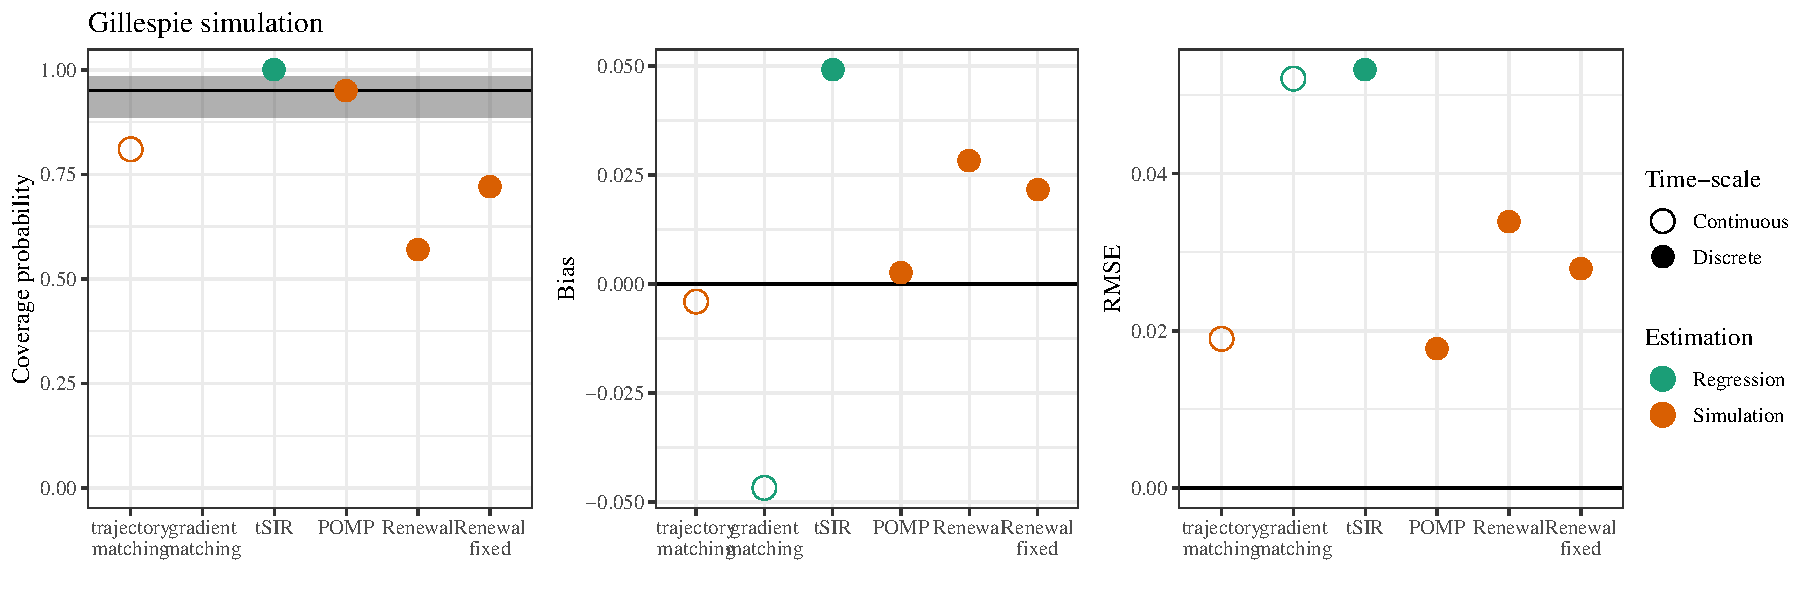
\includegraphics[width=\textwidth]{../figure/compare_estimate_sir.pdf}
\caption{
\textbf{Comparison of the estimates of a constant transmission rate from different method.}
The triangles represent raw TSIR estimates before correcting for the discretization of a continuous-time model.
The black lines show nominal coverage, zero bias, and zero RMSE, respectively.
The grey bars represent the 95\% binomial confidence intervals for 100 simulations.
}
\label{fig:coverage}
\end{figure}

First, we use 100 Gillespie simulations with constant transmission rate (without natural birth or death) to assess the performance of each method to estimate the transmission rate of $\beta$.
Trajectory matching and Sequential Monte Carlo estimate the transmission rate $\beta$, reporting rate $\rho$, over-dispersion parameter $\tsub{\phi}{obs}$, and the initial number of infected individuals $I(0)$ (initial number of the susceptible individual is assumed to be $N - I(0)$).
The renewal equation estimates an additional parameter $\tsub{G}{var}$, which is the approximate variance of the generation-interval distribution.
On the other hand, gradient matching and TSIR estimate only the transmission rate $\beta$.
True susceptible dynamics and reporting are assumed to be known for both methods because they cannot be estimated for a single outbreak with a regression.

Estimates of the transmission rates are summarized into coverage probability, bias, and root mean squared error (RMSE).
Coverage probability is the proportion of confidence intervals that contain the true value over repeated experiments. 
For example, the 95\% confidence interval should contain the true value 95\% of the time.
Bias and RMSE are computed on a log scale.

We find that the Monte Carlo methods (whether the model is represented as a compartmental model or a renewal equation) provide best estimates (\fref{coverage}).
Estimates of the transmission rates based on Sequential Monte Carlo give good coverage and has the least bias and RMSE.
However, in order for the renewal equation model to attain nominal coverage, the simulation time step $\Delta t$ has to be as fine as one-twentieth of the mean generation length; 
simulating an epidemic at one-tenth of the mean generation length results in \swp{70\%} coverage (\swp{see Appendix}).
While trajectory matching can fit a continuous-time model without having to rely on a discretization process, it gives a slightly lower coverage than the nominal probability.

Both regression-based methods (gradient matching and TSIR regression) perform similarly in terms of RMSE.
Gradient matching and TSIR give slightly biased estimates in opposite directions.
Surprisingly, the TSIR regression gives 100\% coverage if we assume that we know the exact susceptible dynamics.
However, the true coverage is likely to be lower because true dynamics of the susceptible population is never exactly known.
Low coverage of the gradient matching method is likely driven by not accounting for uncertainty during the initial smoothing process; we do not explore this idea here.
Finally, we note the summary statistics for the TSIR method are based on corrected estimates; using raw estimates of the transmission rate obtained from the TSIR regression, without correcting for discretization, gives estimates with strong bias and low coverage.

\subsection{Simulation study: estimating time-varying transmission rates}

\begin{figure}[!t]
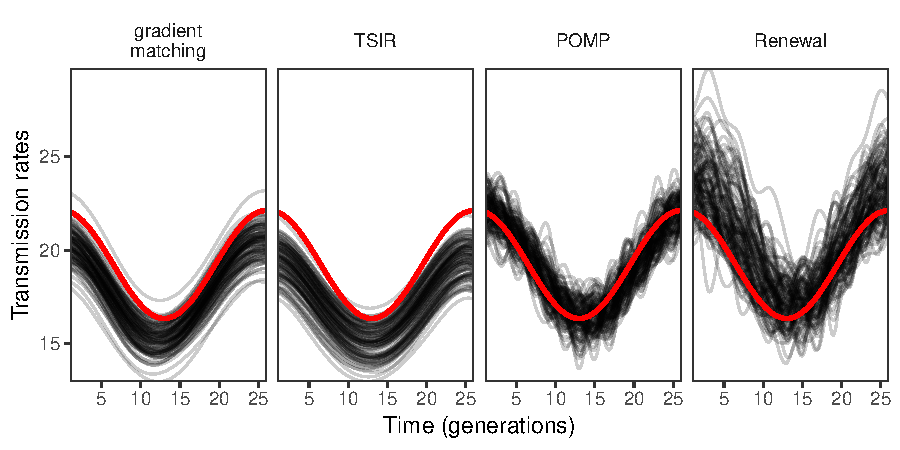
\includegraphics[width=\textwidth]{../figure/compare_transmission.pdf}
\caption{
\textbf{Comparison of the estimates of a time-varying transmission rate from different method.}
The red line represents the true transmission rates.
The black lines represent the estimated transmission rates from 100 simulations.
}
\end{figure}
 
Finally, we use 100 Gillespie simulations with sinusoidal transmission rates to assess the performance of each method to estimate the transmission rate.
We excluded trajectory matching from this analysis because fitting a deterministic model to a time series that is driven by highly nonlinear and stochastic system is difficult and not likely to result in useful inference.
We find that both regression-based methods are able to recover the true shape of the transmission rate reasonably well but give biased estimates.
TSIR method yields a slightly more variable estimates; this is likely to be driven by inaccuracy in the estimates of the reporting rate. 

Monte Carlo methods give more variable estimates.
Estimates generally follow a sinusoidal shape -- transmission rates are higher near the boundaries and lower in the middle -- but are `wigglier'.
Fitting the renewal equation gives much more variable estimates of the transmission rates because the renewal equation accounts for extra uncertainty in the system by allowing for the variance of the generation-interval distribution to vary.
These results suggest that small changes in the transmission rate are difficult to identify in the presence of process error.
In fact, we find similar patterns when we try to fit the TSIR model without using splines \swp{Appendix}.
It is also possible that we may not have enough power to estimate the true shape of the transmission rates from 9 years of data (equivalent to 234 data points assuming biweekly reporting).

\section{Discussion}

Estimating biologically realistic parameters of a model is central to the analysis of epidemic time series.
Here, we compare several different methods for estimating the unobserved transmission rates of the SIR model for recurrent epidemics.
Simple methods that do not make an explicit distinction between different sources of errors (e.g., process and observation error) give reasonable estimates but fail to capture uncertainty associated with their estimates.
More sophisticated methods that explicitly account for these errors provide good estimates.
However, as we increase the flexibility of the model (e.g., by allowing for the shape of the generation-interval distribution to vary), it becomes more difficult to estimate the true shape of the transmission rates.
The TSIR method works reasonably well under several strong assumptions.

\subsection{Discretization}

Fitting a continuous-time stochastic model to an epidemic time series is practically impossible.
Many inferential frameworks rely on discrete-time approximations instead to estimate the parameters of the corresponding continuous-time model \citep{finkenstadt2002stochastic, king2015statistical, champredon2018two, li2018fitting}.
However, the effects of these discrete-time approximations are rarely discussed.
We show that the discretization of a continuous-time model can make a huge difference in the inference.
In particular, the renewal equation has low coverage (\swp{approx70\%}) when the simulation time step is one-tenth of the mean generation time.

The low coverage is likely to be driven by changes in the underlying generation-interval distribution.
As the discretization time step changes, mean and variance of the distribution also changes even when the parameters of the distributions are held constant.
For our example, changing the time step from one-twentieth of the mean generation time to one-tenth increases the mean generation time by 2.5\%.
This change is sufficient to introduce a small bias in our estimates and reduce coverage \swp{Appendix}.
Using a coarser time scale will introduce greater bias and 


\subsection{Generation-interval distributions}


\subsection{Process and observation error}

For weakly non-linear systems with large observation error, 


\subsection{Penalization}



\section{Appendix}

\subsection{Relating incidence, mortality, and prevalence}

First, recall that mortality case can be written as
\begin{equation}
\int_{t-\tsub{t}{rep}}^{t} \gamma I ds.
\end{equation}
When reporting period is equal to mean generation time, i.e., $\tsub{t}{rep} = 1/\gamma$, 
it follows that:
\begin{equation}
\int_{t-\tsub{t}{rep}}^{t} \gamma I ds \approx \gamma I(t-\tsub{t}{rep}) \tsub{t}{rep} = I(t-\tsub{t}{rep})
\end{equation}
Likewise, we can derive a similar relation for incidence:
\begin{equation}
\begin{aligned}
I(t+\tsub{t}{rep}) &= I(t) + \int_{t}^{t+\tsub{t}{rep}} \frac{dI(s)}{ds} ds\\
&= I(t) + \int_{t}^{t+\tsub{t}{rep}} \beta(s) S \frac{I}{N} ds - \int_{t}^{t+\tsub{t}{rep}}\\
&\approx \int_{t}^{t+\tsub{t}{rep}} \beta(s) S \frac{I}{N} ds
\end{aligned}
\end{equation}
Here, we assumed that individuals leaving infected class $I$ from natural mortality is negligible over the reporting period.

\swp{TODO}


\section{Fitting continuous models}

\subsection{Gradient matching}

\begin{figure}[t]
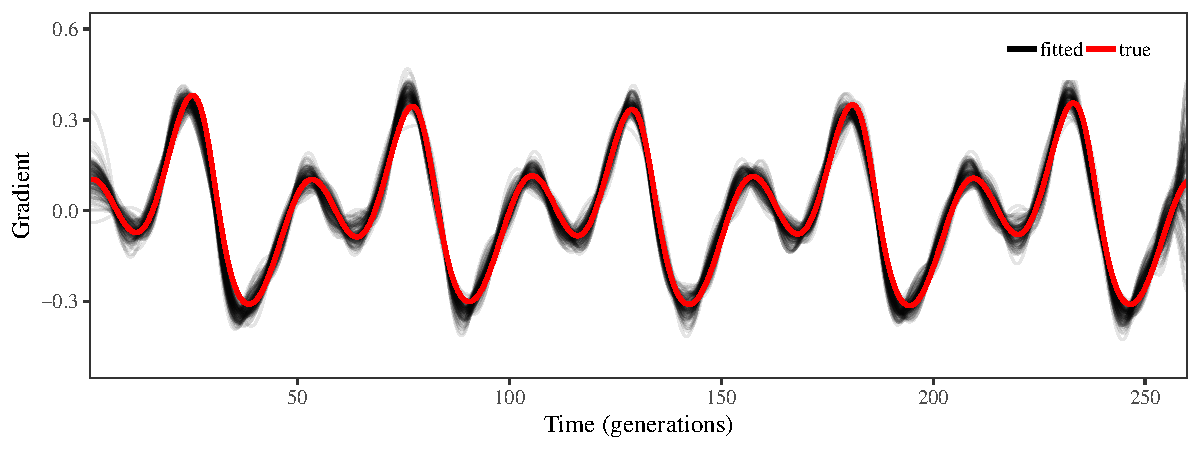
\includegraphics[width=\textwidth]{../figure/gradient_matching_sinusoidal.pdf}
\caption{This is not a caption.}
\end{figure}

Conditions:
\begin{itemize}
	\item See Jost and Ellner (???)
	\item sampled sufficiently
	\item not too much error
	\item Brunel Parameter estimation of ODE’s via nonparametric estimators
\end{itemize}


%% read pomp-Astic somewhere

\subsection{Spectral matching}

What is this? Read Reuman et al. 2006
%% https://www.pnas.org/content/pnas/103/49/18860.full.pdf


\bibliography{thesis}

\pagebreak

\section{Appendix}

\subsection{Derivation of growth rate in discrete-time SIR model}


Derivation:
\begin{equation}
\begin{aligned}
S_{t+\Delta t} &= S_t - S_t (1- \exp(-\beta I_t \Delta t/N))\\
I_{t+\Delta t} &= S_t (1- \exp(-\beta I_t \Delta t/N)) + I_t - I_t (1- \exp(-\gamma \Delta t))
\end{aligned}
\end{equation}
Assuming tat $S_t$ is approximately equal to $N$, we get
\begin{equation}
I_{t+\Delta t} = N_t (1- \exp(-\beta I_t \Delta t/N)) + I_t \exp(-\gamma \Delta t)
\end{equation}
When $I_t \approx 0$, $\exp(-\beta I_t \Delta t/N) \approx 1 - \beta I_t \Delta t/N$ and so
\begin{equation}
\begin{aligned}
I_{t+\Delta t} &\approx  I_t \beta \Delta t + I_t \exp(-\gamma \Delta t)\\
&= I_t (\beta \Delta t + \exp(-\gamma \Delta t))
\end{aligned}
\end{equation}
Substituting $\hat{\gamma}$, we get
\begin{equation}
I_{t+\Delta t} = I_t \left(1 + \beta \Delta t - \frac{\Delta t}{\mu}\right),
\end{equation}
Therefore,
\begin{equation}
I_{t} = I_0 \left(1 + \beta\Delta t - \frac{\Delta t}{\mu}\right)^{t/\Delta t}
\end{equation}
and the initial growth rate is given by
\begin{equation}
r = \frac{1}{\Delta t} \log \left(1 + \beta \Delta t - \frac{\Delta t}{\mu}\right).
\end{equation}




\subsection{Probability of infection}

In both the TSIR model and the hazard-based model, transition from the susceptible comparment, $S$, to the infected compartment, $I$, is represented as a product of number of susceptible individuals and probability of infection between two time steps $t$ and $t + \Delta t$.
The TSIR model assumes that the probability of infection is a linear function of prevalence $I_t$.
This formulation is based on the Euler approximation to the solution of the ordinary differential equation.
On the other hand, the hazard-based model assumes that the probability of infection is an inverse exponential function of prevalence $I_t$.
Besides their differences in the relationship between prevalence and probability of infection, there are two more assumptions that we need to consider: (1) force of infection remains constant over two time steps and (2) new susceptible individuals have zero probability of infection between the two time steps.



\subsection{Infectious period}

Geometric distribution with probability of $1-\exp(-\gamma \Delta t)$ and unit of $\Delta t$.
Then, mean infectious period and generation interval is given by 
\begin{equation}
\frac{\Delta t}{1-\exp(-\gamma \Delta t)}.
\end{equation}
An important but often overlooked component is the variance of the distribution.
Squared coefficient of variation for this distribution is equal to $\exp(-\gamma \Delta t)$, which necessarily depends on pre-specified time-step $\Delta t$.
If we want to match the mean of the distribution to a fixed value $\mu$ regardless of our choices of $\Delta t$, we obtain 
\begin{equation}
\hat \gamma = - \frac{1}{\Delta t} \log\left(1 - \frac{\Delta t}{\mu}\right)
\end{equation}
Then,
\begin{equation}
\mathrm{CV}_{\tiny\textrm{Infectious period}}(\Delta t)^2 = 1 - \frac{\Delta t}{\mu}.
\end{equation}

We expect changes in variation in infectious period to affect variation in stochstic realizations.

This means that the relationship between $r$ and $\mathcal R$ changes.
For this generation-interval distribution, we have
\begin{equation}
\mathcal R = 1 + \frac{\exp(r) -1}{(1-\exp(-\gamma \Delta t)) }
\end{equation}
Substituting 
\begin{equation}
r = \frac{1}{\Delta t} \log \left(1 + \beta \Delta t - \frac{\Delta t}{\mu}\right),
\end{equation}
as well as $\hat \gamma$, we get
\begin{equation}
\mathcal R = 1 + \frac{\mu}{\Delta t} \left(1 + \beta \Delta t - \frac{\Delta t}{\mu}\right)^{1/\Delta t}
\end{equation}
Then, we can obtain a relationship between $\mathcal R$ of a discrete-time system and that of a corresponding continuous time system, assuming that contact rate $\beta$ and mean generation-time $\mu$ are the same:
\begin{equation}
\mathcal R_{\tiny \textrm{discrete}} = 1 + \frac{\mu}{\Delta t} \left(1 + \frac{(\mathcal R_{\tiny \textrm{continuous}}  - 1) \Delta t }{\mu}\right)^{1/\Delta t}
\end{equation}

On the other hand, we may want to match choose $\beta$ and $\mu$ to match true $r$ and $\mathcal R$.

\end{document}
